% !TEX encoding = UTF-8 Unicode
%!TEX root = thesis.tex
% !TEX spellcheck = en-US
%%=========================================
\chapter{Architecture}
\label{chapterArchitecture}

The architecture, and especially communication between services, is important when creating microservices, as this largely determines the maintainability, efficiency, and modularity of the system.
Choosing a suiting architecture is therefore very important.

\section{System architecture}
When building a microservice based system, it is important to consider the granularity of the services \citep{granularity}. A coarse grained interface was chosen, i.e. each service receives and sends \acrshort{json} structured information. The goal of each service is to have a well-defined function and that each microservice consists of components that are easy to reuse. By making each service have a well-defined function, a loose-coupling between the services can be maintained.

Without loose coupling, modifying a service often necessitates modifying all services that interacts with it. This can become a problem in monolithic and to an extent service-oriented architectures, because of their unclear guidelines for separating services \citep{ibmSoaDescription}.

This system consists of eight microservices. They are described in section \ref{sec:microservices}, and the architecture shown in figure \ref{fig:fullarkitektur}. One of the services has two implementations, in two different programming languages, in order to show how a service could easily be replaced in the microservice architecture. The status service is not shown in figure \ref{fig:fullarkitektur}, as it performs monitoring, and is not part of the \acrshort{cms} system.


\begin{figure}[H]
    \centering
     \includegraphics[scale=0.4]{fig/architecture/system-architecture}
    \caption{Connections between different microservices and other components.}
\end{figure}\label{fig:fullarkitektur}

\section{How the services communicate}
A \acrshort{dht} works by distributing the responsibility for maintaining the mapping from keys to values among the nodes in the network. As  mentioned in section \ref{subsec:alternative_arch}, this property is exploited to store the type of service and the \acrshort{ip} addresses associated with that type. This also automatically distributes the load among all nodes, and by doing so fulfils NFR-5.

The node is divided into two parts: one part for communicating with the other nodes in the network, and one part which exposes a \acrshort{rest} \acrshort{api} to the service, so that it can easily query the network for \acrshort{ip} addresses.

This removes the need for creating language specific bindings, and makes the node easier to test, as \acrshort{http} requests are sufficient to obtain data from a given node. Each service runs a node as a part of the microservice.

When a service $A$ wants to communicate with another service of type $B$, it begins by querying the node to obtain an \acrshort{ip} address to a node $C$ of type $B$. This allows service $A$ to communicate directly with $C$. If $A$ detects that $C$ does not respond, it simply removes $C$ from the list of available services. This flow is illustrated in figure \ref{fig:comm_example}
\begin{figure}[H]
    \centering
    \includegraphics[scale=0.30]{fig/architecture/communication-example}
    \caption{Flow of requests during a query.}\label{fig:comm_example}
\end{figure}

\section{The architecture of each microservice}\label{sec:microservices}

Originally there were five microservices related to the creation and publishing of content: editor, publishing, datasets, administration, and template service. These would form the core of the system. Figure \ref{fig:content_arch} shows an overview of their architecture.

It was however decided that the datasets and administration services would be unnecessary for the purpose of demonstrating the microservice architecture, so they were excluded.

It was also decided that having all the microservices supply their own front-end would be cumbersome and unnecessary, because many of them had very small or no front-end at all. So instead, all the front-ends were merged into a unified front-end service. The editor turned out to not need its own back-end at all, so it was entirely merged into the front-end service. An overview of the new content architecture is shown in \ref{fig:content_arch_new}.

\begin{figure}[H]
    \centering
    %\includegraphics[scale=0.20]{fig/architecture/content}
    \scalebox{0.8}{\pgfdeclarelayer{background}
\pgfdeclarelayer{foreground}
\pgfsetlayers{background,main,foreground}

\tikzstyle{object}=[draw, text width=5em, 
    text centered, minimum height=2.5em]

\tikzstyle{DB}=[draw, text width=2em, 
    text centered, minimum height=2em,circle]
%\tikzstyle{user}=[draw, text width=7em,
%    text centered, minimum height=2em,diamond]
\tikzstyle{user}=[draw=none]

\begin{tikzpicture}    
    \node[user] (admin) {Administrator};
    \node[object] (admin_front) [below=of admin] {Admin front-end};
    \node[object] (admin_back) [below=of admin_front] {Admin back-end};
    \node[DB] (admin_db) [left=of admin_back] {DB};

    \node[object] (publish_back) [right=2cm of admin_back] {Publisher back-end};
    \node[object] (publish_front) [above=of publish_back] {Publisher front-end};
    \node[DB] (publish_db) [below=of publish_back] {DB};

    \node[object] (editor_back) [right=2cm of publish_back] {Editor back-end};
    \node[object] (editor_front) [above=of editor_back] {Editor front-end};

    \node[object] (templates) [right=2cm of editor_back] {Templates};
    \node[DB] (templates_db) [right=of templates] {DB};

    \coordinate (mid) at ($(publish_front)!0.5!(editor_front)$);
    \node[user] (employee) [above=2cm of mid] {Employee};

    \node[object] (datasets_front) [right=1cm of employee] {Datasets front-end};
    \node[object] (datasets_back) [right=of datasets_front] {Datasets back-end};
    \node[DB] (datasets_db) [right=of datasets_back] {DB};


    \draw[<->,thick] (admin) -- (admin_front);
    \draw[<->,thick] (admin_front) -- (admin_back);
    \draw[<->,thick] (admin_back) -- (admin_db);
    \draw[<->,thick] (admin_back) -- (publish_back);
    \draw[<->,thick] (publish_back) -- (publish_db);
    \draw[<->,thick] (publish_back) -- (publish_front);
    \draw[<->,thick] (editor_back) -- (publish_back);
    \draw[<->,thick] (editor_back) -- (editor_front);
    \draw[<->,thick] (templates) -- (editor_back);
    \draw[<->,thick] (templates) -- (templates_db);
    \draw[<->,thick] (employee) -- (publish_front);
    \draw[<->,thick] (employee) -- (editor_front);
    \draw[<->,thick] (employee) -- (datasets_front);
    \draw[<->,thick] (datasets_front) -- (datasets_back);
    \draw[<->,thick] (datasets_back) -- (datasets_db);

    \def\FILL{blue!20}
    %\def\FILL{yellow!20}
    %\def\FILL{none}
    \begin{pgfonlayer}{background}
        \path (admin_front.north -| admin_db.west)+(-0.5,0.3) node (a) {};
        \path (admin_db.south -| admin_back.east)+(+0.3,-0.2) node (b) {};
        \path[fill=\FILL, 
            rounded corners, draw=black!50, dashed]
            (a) rectangle (b);


        \path (publish_front.north -| publish_front.west)+(-0.5,0.3) node (a) {};
        \path (publish_db.south -| publish_db.east)+(+0.8,-0.2) node (b) {};
        \path[fill=\FILL,
            rounded corners, draw=black!50, dashed]
            (a) rectangle (b);

        \path (editor_front.north -| editor_front.west)+(-0.5,0.3) node (a) {};
        \path (editor_back.south -| editor_back.east)+(+0.3,-0.2) node (b) {};
        \path[fill=\FILL, 
            rounded corners, draw=black!50, dashed]
            (a) rectangle (b);

        \path (templates.north -| templates.west)+(-0.5,0.3) node (a) {};
        \path (templates.south -| templates_db.east)+(+0.3,-0.2) node (b) {};
        \path[fill=\FILL, 
            rounded corners, draw=black!50, dashed]
            (a) rectangle (b);

        \path (datasets_front.north -| datasets_front.west)+(-0.5,0.3) node (a) {};
        \path (datasets_front.south -| datasets_db.east)+(+0.3,-0.2) node (b) {};
        \path[fill=\FILL, 
            rounded corners, draw=black!50, dashed]
            (a) rectangle (b);


    \end{pgfonlayer}
\end{tikzpicture}
}
    \caption{Overview of the original design of the content services.}\label{fig:content_arch}
\end{figure}

\begin{figure}[H]
    \centering
    \scalebox{0.8}{\input{fig/architecture/tcontent_new}}
    \caption{Overview of the refactored design of the content services.}\label{fig:content_arch_new}
\end{figure}

The search microservice was also changed. Originally, it was supposed to be a single microservice -- but the team responsible for implementing it decided to split it into three microservices, as it would otherwise have to be larger than first anticipated.

\subsection{Front-end service}
The front-end of the project uses Django to render the pages according to templates. This service works by asking other services for content and displaying it to the user in its proper template. By having one service render all of the visible content, it is easy to change the overall look and feel without having to change more than one service. It also uses some JavaScript to implement Summernote as the \acrshort{wysiwyg} editor. 

\subsection{Publishing service}
The publishing service provides an \acrshort{http} \acrshort{api} to store and retrieve articles and information about articles, and to get a list of currently stored articles. It works by assigning a unique identifier to articles when they are inserted, which can then be used to fetch or delete articles. Each article is stored as a \acrshort{json} object with fields for the article body and various information about the article.

The Publishing service is implemented twice. One implementation is written in using Node.js and the express.js web framework, the other is written in Python using the Django web framework. Both implementations use MongoDB to store the articles, since a simple key/value store for mapping IDs to \acrshort{json} objects is all that is needed.

\subsection{Template service}
In order to make it easy to add, remove, or get a template, a dedicated service for template management was created.
This service is written in Go, and uses MongoDB to store templates. MongoDB was choosen because a key/value store was sufficient, since only the name of the template and the \acrshort{html} associated with each template was going to be stored.

The service provides an \acrshort{api} which can be used to obtain and manage the templates in the database. The \acrshort{api} was implemented using the web framework library Gin, which makes creation of web applications easy.

\subsection{Status services}
To have an overview of the status of each service, a status service was made. The service uses \acrshort{http} to try to get a specific resource on one of the services, to verify that the service responds to queries. In addition, it links to the documentation for the service.

\subsection{Authentication service} \label{subsec:authServiceArchitecture}
Microauth is the service used as the authentication service. It is made using Python and Django, implementing OAuth2. The service wraps around an implementation of OAuth2, and handles registering, authentication, and authorisation by providing an \acrshort{api} for communication. Any client will communicate through the OAuth2 provider either directly or indirectly, by passing tokens as part of their requests. The tokens are mapped to users and will therefore make sure to provide whatever content is available to the users. 

There are also tokens set up between the services themselves, as confidential tokens, which connects and authenticates the services between each other -- so they know they can trust each other, therefore preventing fraudulent services from entering the network as a man in the middle.

\begin{figure}[H]
    \centering
      \begin{sequencediagram}
  \newthread{A}{Client}{}
    \newinst[2.5]{B}{Resource Owner}{}
    \newinst[1]{C}{Authorisation Server}{}
    \newinst[1]{D}{Resource Server}{}
    \begin{call}{A}{(A) Authorisation Request}{B}{(B) Authorisation Grant}
      \postlevel
    \end{call}
    \begin{call}{A}{(C) Authorisation Grant}{C}{(D) Access Token}
      \postlevel
    \end{call}
    \begin{call}{A}{(E) Access Token}{D}{(F) Protected Resource}
      \postlevel
    \end{call}
  \end{sequencediagram}

    \caption{The flow of OAuth2 is as described in the OAuth2 \acrshort{rfc} \citep{oauth2RFC}, section 1.2. }\label{fig:oauth-flow}
\end{figure}

\subsection{Index service}
The index service provides keyword based retrieval of documents. It is notified by the publishing service whenever an article is published or modified, and updates its mapping appropriately. When queried with a keyword, the service returns a list of articles containing it. The index service also provides additional information about keywords, such as frequencies and completion lists. 

The index service is implemented in Python, and uses the Twisted networking engine \citep{twisted}.

\subsection{Spelling service}
The spelling service is queried with an individual word. It has two functions -- spelling correction and word completion. 
If the query concerns spelling correction, the service consults a frequency word list and uses edit distances to find possible candidates for correction. 
If the query concerns completion of the query word -- for instance in the use case of typing queries in search boxes, where the last word in the query is only partially completed -- the service consults its word list, returning possible completions ranked by frequency. 
Both generic and content-specific spelling feedback is supported, through the use of multiple frequency lists.

The spelling service is implemented in Python, using the networking library Twisted. It also uses a probabilistic model from Norvig for finding words within specific edit distances of the query \citep{norvig}.

\subsection{Search service}
The search service's area of responsibility is to return lists of documents to users, as a response to search queries. Users make requests through a search front-end, which conveys queries to the search back-end via its exposed \acrshort{api}.

The search back-end communicates with the index and with the spelling service.
The index service is queried for articles matching keywords in the user-supplied query, while the spelling service is queried for feedback to the user on potentially mistyped or incomplete words.

The back-end is implemented in Python, using the networking library Twisted. 
The Python Natural Language Toolkit \citep{nltk} is used for stemming and ignoring stopwords, which have minimal value for searches.

Figure \ref{fig:search_arch} shows the sequence of calls during a normal search. 
The user submits a query through the search front-end to the search back-end, and the index is consulted for a list of matching documents for each keyword in the query. 
The search back-end may then retrieve and rank the documents in the list from the index.

The back-end also consults the spelling service for spelling corrections, the spelling service constructing a list of candidates for each keyword in the query not recognised as a valid word. 
The search back-end returns both the results and the list of spelling feedback.



\begin{figure}[H]
    \centering
    %\documentclass{standalone}
%\usepackage[utf8]{inputenc}
%\usepackage{tikz}
%\usepackage{tikz-qtree}
%\usepackage{enumitem}
%\usepackage{pdfpages}
%\usepackage{amsmath}
%\usepackage{graphicx}
%\usepackage{tikz}
%\usepackage{pgf}
%\usepackage{pgf-umlsd}

%\usetikzlibrary{arrows,positioning,calc,shapes,fit}

%\begin{document}
  \begin{sequencediagram}
  \newthread{A}{Search front-end}{}
    \newinst[2]{AA}{Search back-end}{}
    \newinst[2]{B}{Spelling service}{}
    \newinst{C}{Index service}{}
    \begin{call}{A}{Search(query)}{AA}{\{results:[...], spell:[[...], ...]\}}
      \begin{sdblock}{Loop}{Foreach keyword}
        \begin{call}{AA}{matches()}{C}{[r1, r2, ..., rn]}
        \end{call}
      \end{sdblock}
      \begin{sdblock}{Loop}{Foreach keyword}
        \begin{call}{AA}{correction()}{B}{[c1, c2, ..., cn]}
          \begin{sdblock}{Condition}{if uncached}
            \begin{call}{B}{frequencies()}{C}{\{...\}}
            \end{call}
          \end{sdblock}
        \end{call}
      \end{sdblock}
    \end{call}
    
  \end{sequencediagram}
%\end{document}

    \caption{Sequence diagram of a complete search query. A list of results and a list of lists of spelling feedback (indexed by position in query sentence) is returned.}
    \label{fig:search_arch}
\end{figure}

Not shown is the sequence of calls for partial searches; partial searches do not return any results beyond spelling feedback. For partial searches, the sub-list corresponding to the positionally last word in the query is a list of possible keyword completions rather than corrections. The remaining sub-lists are the usual corrections. 

\section{How the architecture scales}\label{sec:architecture-scalability}
% Sklirg can help when some keywords are defined.
% Yay!
Figure \ref{fig:frontend-scaling} illustrates how adding more instances of the front-end service improves the overall response time of the service, thus showing how the system scales. The service was tested using Siege, which is a \acrshort{http} load testing and benchmarking tool \citep{siege}. Siege was used to simulate 250 simultaneous users which requested the frontpage every second for 15 seconds. In order to see whether the response times were consistent, Siege was ran three times so that the data from each run could be compared.
The server used to run the system was a DigitalOcean droplet with 4GB of RAM and two CPU cores.
\begin{figure}[H]
    \centering
    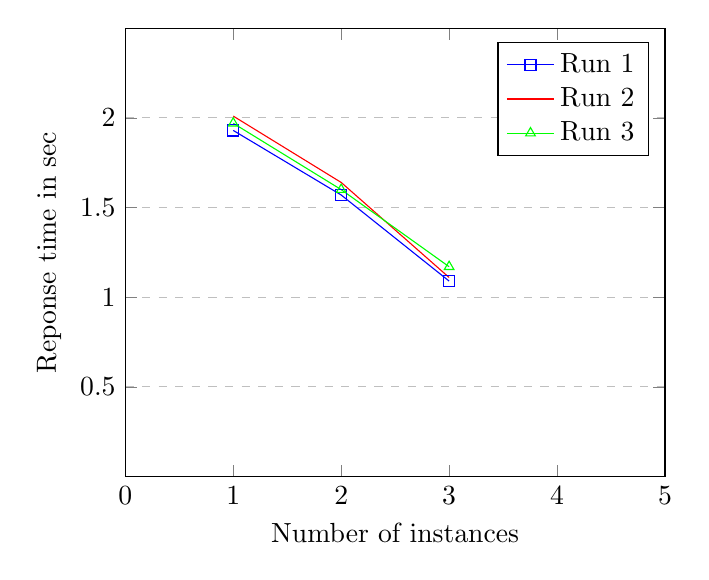
\begin{tikzpicture}
\begin{axis}[
    xlabel={Number of instances},
    ylabel={Reponse time in sec},
    xmin=0, xmax=5,
    ymin=0, ymax=2.5,
    xtick={0, 1,2,3,4,5},
    ytick={0.5, 1, 1.5, 2},
    legend pos=north east,
    ymajorgrids=true,
    grid style=dashed,
]
 
\addplot[
    color=blue,
    mark=square,
    ]
    coordinates {
    (1, 1.93)(2, 1.57)(3, 1.09)
    };
    \addlegendentry{Run 1}
\addplot[
    color=red,
    mark=circle,
    ]
    coordinates {
    (1, 2.01)(2, 1.64)(3, 1.11)
    };
    \addlegendentry{Run 2}
\addplot[
    color=green,
    mark=triangle,
    ]
    coordinates {
    (1, 1.97)(2, 1.60)(3, 1.17)
    };
    \addlegendentry{Run 3}
 
\end{axis}
\end{tikzpicture}
    \caption{The scalability of the front-end service}\label{fig:frontend-scaling}
\end{figure}

Figure \ref{fig:publishing-scaling} shows how the publishing services scales when adding more instances. The same exact setup as above was also used to test this service. As figure \ref{fig:frontend-scaling} and \ref{fig:publishing-scaling} shows, the system scales relatively linearly. 
\begin{figure}[H]
    \centering
    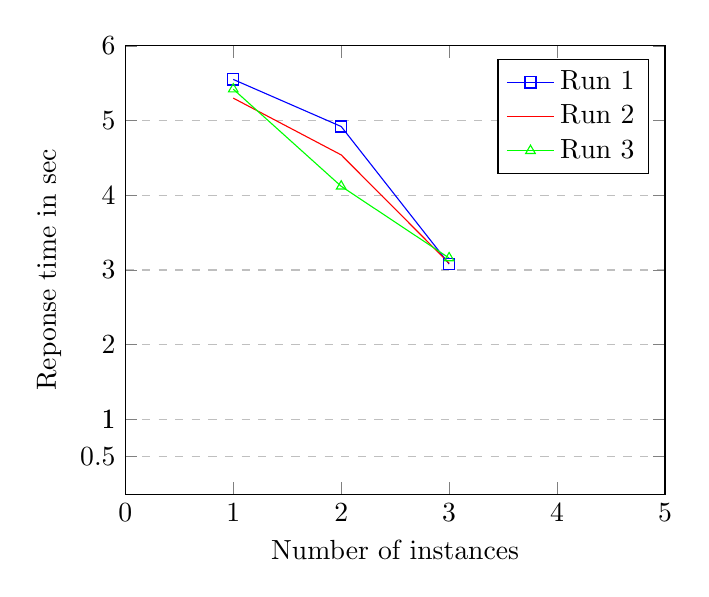
\begin{tikzpicture}
\begin{axis}[
    xlabel={Number of instances},
    ylabel={Reponse time in sec},
    xmin=0, xmax=5,
    ymin=0, ymax=6,
    xtick={0, 1,2,3,4,5},
    ytick={0.5, 1, 1, 2, 3, 4, 5, 6},
    legend pos=north east,
    ymajorgrids=true,
    grid style=dashed,
]
 
\addplot[
    color=blue,
    mark=square,
    ]
    coordinates {
    (1, 5.55)(2, 4.92)(3, 3.08)
    };
    \addlegendentry{Run 1}
\addplot[
    color=red,
    mark=circle,
    ]
    coordinates {
    (1, 5.30)(2, 4.54)(3, 3.09)
    };
    \addlegendentry{Run 2}
\addplot[
    color=green,
    mark=triangle,
    ]
    coordinates {
    (1, 5.42)(2, 4.12)(3, 3.16)
    };
    \addlegendentry{Run 3}
 
\end{axis}
\end{tikzpicture}
    \caption{The scalability of the publishing service}\label{fig:publishing-scaling}
\end{figure}

The performance of the system is significantly better when dealing with 100 users making 50 \acrshort{rps}, which according to non-functional requirement NFR-1 is the normal load. Figure \ref{fig:normal-load} shows how one instance of the front-end service performs under normal load. The average response time is 0.25 seconds, which fulfils NFR-1. Siege was used to simulate 100 simultaneous users making requests every 1-3 seconds for one minute, which is equivalent to a load of approximately 50 \acrshort{rps}.
\begin{figure}[H]
    \centering
    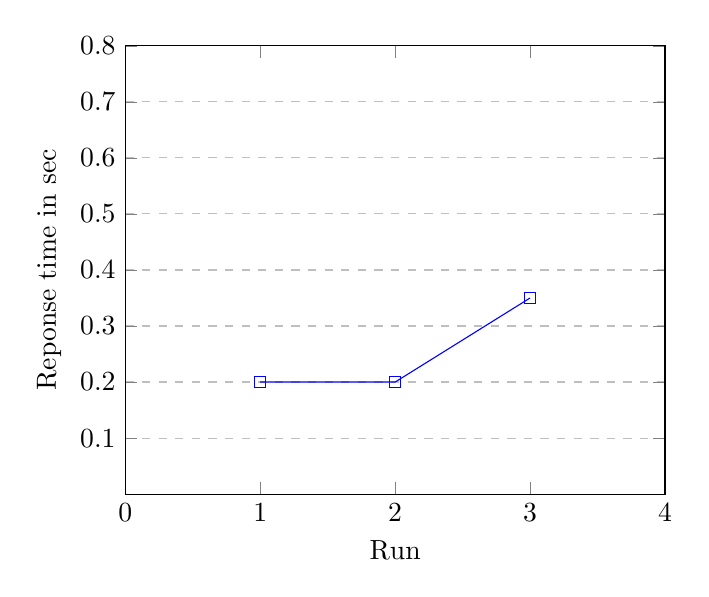
\begin{tikzpicture}
\begin{axis}[
    xlabel={Run},
    ylabel={Reponse time in sec},
    xmin=0, xmax=4,
    ymin=0, ymax=0.8,
    xtick={0, 1,2,3,4,5},
    ytick={0.1, 0.2, 0.3, 0.4, 0.5, 0.6, 0.7, 0.8},
    legend pos=north east,
    ymajorgrids=true,
    grid style=dashed,
]
\addplot[
    color=blue,
    mark=square,
    ]
    coordinates {
    (1, 0.20)(2, 0.20)(3, 0.35)
    };
 
\end{axis}
\end{tikzpicture}
    \caption{The performance of the front-end service under normal load}\label{fig:normal-load}
\end{figure}

\subsection{Stress testing}\label{subsec:stress-testing}
Figure \ref{fig:stress-testing} shows how the system handles an increasing amount of users. The response time increases linearly with the amount of users. Siege was used to simulate the users. Each user requested the site every 1-3 seconds for 30 seconds. The delay at 750 users is noticeable, but it would be easy to add new instances of the service in order to reduce the response time.
\begin{figure}[H]
    \centering
    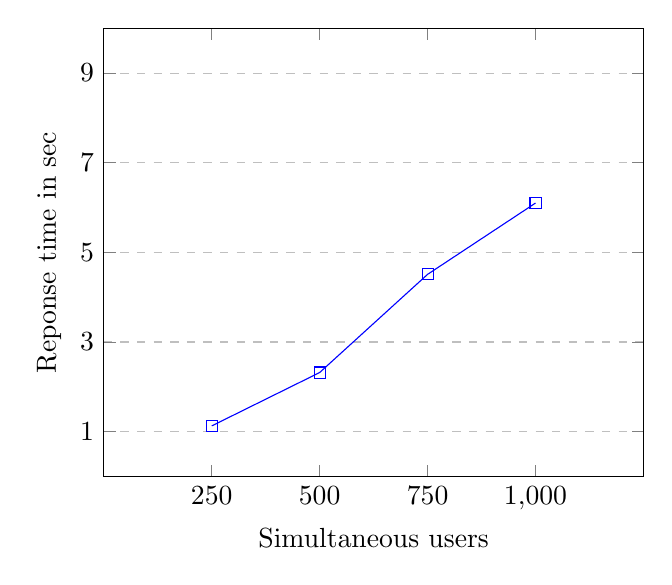
\begin{tikzpicture}
\begin{axis}[
    xlabel={Simultaneous users},
    ylabel={Reponse time in sec},
    xmin=0, xmax=1250,
    ymin=0, ymax=10,
    xtick={250, 500, 750, 1000},
    ytick={1, 3, 5, 7, 9},
    legend pos=north east,
    ymajorgrids=true,
    grid style=dashed,
]
\addplot[
    color=blue,
    mark=square,
    ]
    coordinates {
    (250, 1.13)(500, 2.32)(750, 4.51)(1000, 6.1)
    };
 
\end{axis}
\end{tikzpicture}

    \caption{How the front-end service performs under stress}\label{fig:stress-testing}
\end{figure}

\section{Deployment}
Each instance of a microservice is deployed in a Docker container. This makes it easy to add new instances of each microservice, and services can be upgraded by simply replacing the container.
Management of containers is also made easy by creating pre-packaged images that can be managed through Docker Compose.
Since each container has separate log files, Logstash is used to collect and store logs. Figure \ref{fig:deploy_arch} shows the overview of how the services are deployed.
\begin{figure}[H]
    \centering
    \includegraphics[scale=0.40]{fig/architecture/deployment-overview}
    \caption{Deployment of services.}\label{fig:deploy_arch}
\end{figure}


\section{How the system could be improved}
Several ways of improving the system was discovered while developing the system. This section describes some of the ideas on how to improve and how they would improve the system.

\subsection{Architecture}
The primary reason for choosing to use a \acrshort{dht} to perform service discovery, was to experiment with an alternative way of performing service discovery. We would not recommend doing this in a production environment, as this is not as mature of a communication architecture as many other service-discovery architectures, it lacks a proper way of recovering from errors, and has little support for health checking.

The implemented method also adds unnecessary complexity to each service, since the entire service has to be updated if the program running the \acrshort{dht} needs to be changed.

We would therefore instead recommend using a different tool such as Consul for this, which is a distributed key-value store. It is fault tolerant and performs extensive health checks. It can also be distributed over multiple servers to avoid a single point of failure \citep{consulMicroservice}.
Consul works similar to the \acrshort{dht} used in this project, i.e.\ by providing a \acrshort{rest} \acrshort{api} that can be used to obtain the \acrshort{ip} address. This means that this system easily could be modified to use Consul instead.

\subsection{Deployment}
One big problem when working with microservices is determining how the data is to be duplicated across the services of the same type. For instance, if one service is used to host articles, how will services of the same type receive articles posted to another service than itself? This was solved by hosting a database separately, and having all the services of a given type connect to the same database.

A better solution would however be to host the databases internally in each service, and having the databases function as a cluster. This would provide redundancy, as well as flexibility through enabling the use of different versions of the same database. It would most likely also lead to a more efficient system, as the data would be stored locally accessible with each service instance. By using clustering the system would improve performance, but it might not be fully up-to-date on data in other clusters. This is a problem that occurs for any clustered system, so the implementation would need to take this into account to achieve data-consistency.

In a larger-scale environment, it would also be a good idea to use a cluster management application such as Mesosphere. Applications like mesosphere are built for handling large-scale microservices and containers \citep{digitalOceanMesosphere}.

\subsection{Services}
\paragraph{The front-end} was implemented as one service, in order to avoid too much complexity and maintain changeability.
One argument for why the front-end should have been split into at least two different services is the fact that if this had been done in a full scale project, one could argue that the architecture of the front-end is more a \acrshort{soa} than it is a microservice architecture.

One of the ways a true microservice architecture could have been achieved even with a larger scale project, would be to have an Angular or React based front-end\footnote{Angular.JS and React.JS are front-end JavaScript frameworks used for interactive web pages.}, rather than Django. This would allow each service to expose its own front-end through its \acrshort{api}. This way, the services would depend less on each other and there would not be any single point of failure.